\documentclass[conference]{IEEEtran}
\IEEEoverridecommandlockouts
% The preceding line is only needed to identify funding in the first footnote. If that is unneeded, please comment it out.
\usepackage{cite}
\usepackage{amsmath,amssymb,amsfonts}
\usepackage{algorithmic}
\usepackage{graphicx}
\usepackage{textcomp}
\usepackage{xcolor}
\usepackage{titlesec}
\usepackage{fancyhdr}
\pagestyle{fancy}
\fancyhf{}
\rfoot{\thepage}
\titleformat{\subsection}{\normalfont\small\bfseries}{\thesubsection}{1em}{}
\renewcommand{\thesubsection}{\thesection.\arabic{subsection}}
\titleformat{\section}{\normalfont\large\bfseries}{\thesection}{1em}{}
\renewcommand{\thesection}{\arabic{section}}

\def\BibTeX{{\rm B\kern-.05em{\sc i\kern-.025em b}\kern-.08em
    T\kern-.1667em\lower.7ex\hbox{E}\kern-.125emX}}
\begin{document}

\title{Game Theoretic Scheduling : A new approach for Real-time Task Scheduling in Cloud Computing\\

}

\author{\IEEEauthorblockN{ Neaz Mahmud}
\IEEEauthorblockA{\textit{Electronics Engineering} \\
\textit{Hamm Lippstadt University Of Applied Science}\\
Lippstadt, Germany \\
Neaz.mahmud@stud.hshl.de}
}

\maketitle

\begin{abstract}
One of the newest technologies in the area of distributed computing is cloud computing, which was created to meet user needs and demands. The virtualization method is used to build a number of virtual machines, which serve as the foundation for cloud computation. One of the main challenges in cloud computing is effective scheduling of tasks and completing their execution prior to the deadline to maximize processor utilization, maximize throughput, and minimize task waiting times.In order to reduce the overall completion time and overall waiting time for real-time tasks in the cloud computing environment,a system model and a game-theoretic framework are proposed in this paper. In the proposed game model, the task assumes the role of a player, the virtual machine assumes the role of a strategy, and the completion time and waiting time are used to represent the player's payoff. The cooperative and non-cooperative game models were used in the experiments. According to the findings of experiments, the cooperative game model has a lower total execution time and total waiting time than the non-cooperative game model.\end{abstract}

\section{\textbf{Introduction}}
\subsection{Cloud Computing}
The most fundamental cloud computing technique is virtualization, which makes it possible to create multiple virtual machines (VMs) on a single physical machine. In other words, cloud computing combines the virtualization method with distributed, traditional high-performance computing. Furthermore, the cloud environment is practical for the deployment of a variety of applications due to its simplicity, availability, and computing power. These tasks are known as real-time tasks because some of them require a response within a specific time frame or deadline. 
\subsection{Challenges}
Although task scheduling is an effective way to boost system performance, the timing constraint makes it difficult to use for real-time tasks. Task scheduling is the process of carrying out tasks (requests) with the few resources (virtual machines) at hand in order to improve a particular system's performance\cite{arunarani2019task}. Without a good scheduling algorithm, resources may be used inefficiently, waiting times may increase, deadlines may be missed, etc. The task scheduling area of cloud computing has seen a lot of work, but the emergence of new applications and technologies makes it an open research problem. Although it may seem like the cloud has endless resources, there are occasionally times when multiple tasks must contend for scarce resources. From the standpoint of the cloud service provider, scheduling must increase revenue regardless of whether tasks compete for resources or resources compete for the task. From the user's perspective, however, the scheduling needs to be done so that the user's needs are met with the least amount of overhead. To accomplish the aforementioned objective, a cloud broker's or scheduler's decision to generate a task-VM pair must be effective and appropriate. In this regard, we can use game theory, a subfield of applied mathematics. 
\subsection{Game theory in cloud computing}
Game theory is the study of how independent, competitive players or decision-makers interact in order to make the best choices\cite{li2014non}. The game model can be cooperative or non-cooperative, depending on the interaction. In this paper, a framework for real-time task scheduling is proposed that takes into account both cooperative and non-cooperative game models. As performance metrics, total completion time and total waiting time are calculated. This paper's main goal is to present a game-theoretic method for allocating real-time tasks in a cloud computing environment. 




The structure of the rest of this paper follows: Literature overviews are presented in Section 2. A brief introduction to cooperative and non-cooperative game theory is provided in Section 3. The proposed system model, which includes the VM model, task model, and scheduling model, is presented in Section 4. Section 5 discusses a game-theoretic framework for real-time task scheduling including Mechanisms' use of both cooperative and non-cooperative games. The experimental results are discussed in Section 6, and Section 7 wraps up the work done in this paper by summarizing it, drawing conclusions, and outlining future work.

\bigskip
\section{Literature Overview}
The issue of task scheduling in the cloud environment has drawn the attention of numerous researchers in recent years. This study concentrated specifically on task scheduling using a game theory model. For the purpose of solving task scheduling issues and achieving energy efficiency in the cloud environment, the author of \cite{yang2020task} has created a cooperative game model. A bottom-up Game-theoretic Task Allocation (BGTA) framework was created by researchers in \cite{zhang2018real} for the distribution of social sensing tasks to non-cooperative edge computing nodes.
They want to maximize the benefits to the edge node while ensuring that applications meet the QoS requirements. In order to match a task with the best machine in cloud manufacturing, Zhang et al. \cite{zhang2017game} used a mathematical model based on game theory. A non-cooperative game model is created for reliability-based task scheduling in the cloud system because reliability is a key component of the cloud system in \cite{li2014non}. In \cite{roungas2019game}, a framework that uses the game theory concept to identify the worst-case scenario in real systems is proposed. Under certain financial restrictions, the author of \cite{samadi2018heft} proposed an improved HEFT algorithm to achieve load balancing across VMs while minimizing makespan. The efficiency of the cooling system is impacted by the thermal imbalance in the data center, which leads to an increase in energy usage. To improve the thermal balance in this situation, Akbar et al. \cite{akbar2019game} proposed a cooperative game-based thermal aware resource allocation. Researchers suggested a two-phase scheduling algorithm in \cite{abrishami2013deadline} to lower the cost of work-flow applications' execution. In \cite{ergu2013analytic}, the author described a task-oriented resource allocation method in which computing resources are assigned based on the task's rank in the pairwise comparison matrix.  However, very few studies focus on real-time task scheduling. In this regard, using a concept from game theory,a scheduling framework for a real-time task is proposed in this paper.

\bigskip
\section{\textbf{Co-operative and Non Cooperative Game Theory}}
In the study of game theory, there are two distinct methods for examining the strategic interactions between decision-making entities: cooperative game theory and Non-cooperative game theory. They differ in how they approach player cooperation, negotiation, and coalition formation. Their distinctive contributions to the study of strategic decision-making can be better understood by diving deeper into their characteristics and methodologies.
\subsection{Co-operative Game Theory}
The focus of cooperative game theory is on circumstances where players can band together or form alliances to achieve win-win results. It looks into the various strategies players can use to maximize their group rewards through cooperation, negotiation, and binding agreements. The stability and efficiency of coalition structures are analyzed using cooperative game theory, which also looks at how players distribute rewards within these coalitions. The core, Shapley value, bargaining solutions, and cooperative solution concepts are important ideas in cooperative game theory. These ideas shed light on how rewards are distributed and how fair outcomes are when players work together. In the theory of cooperative games, it is presupposed that players can cooperate, trust one another, and effectively communicate.\cite{Ichiishi1990Comparative}
\subsection{Non Cooperative Game Theory}
As opposed to cooperative game theory, non-cooperative game theory looks at situations where players act independently and in their own best interests without actively cooperating or forming alliances. It emphasizes strategic interactions in which each participant seeks to maximize their own gains while taking other players' actions and strategies into account. The goal of non-cooperative game theory is to find equilibrium solutions, like the Nash equilibrium, in which no player has a reason to unilaterally depart from their chosen course of action. A key tool for examining strategic interactions in non-cooperative games is the notion of Nash equilibrium. Extensive form games, sub-game perfect equilibrium, dominant strategies, mixed strategies, and mixed strategies are additional key ideas in non-cooperative game theory. According to non-cooperative game theory, players are rational decision-makers who act selfishly and independently without any form of communication\cite{Kamecke1989Non}

\bigskip
\section{\textbf{System Model}}
The system model of the suggested method for real-time task scheduling will be shown in this section. Virtual machine, scheduler, and task are the three main components of a cloud computing system's architecture. The scheduler serves as a bridge between the virtual machine and the tasks. Virtual Machine is in charge of carrying out users' requests (tasks), while User serves as the source of task generator.

\subsection{Virtual Machine Model}
The computing infrastructure for user tasks is provided by a group of virtual machines V = \{v1, v2, \ldots, vm\}
 in the cloud environment. Each virtual machine has its own processing power, or speed of execution j = \{1, 2, \ldots, m\}. The common metric, Million Instructions Per Second (MIPS), is used to assess the virtual machine's computing power.

\subsection{Task Model}
The user generates the task and forwards it to the scheduler. Let $T = \{t1, t2, \ldots, tn\}$ be the collection of independent tasks created by various users.  Each task in T, $t_{i}$, $i = \{1, 2, \ldots, n\}$ is modeled by the following parameters: $t_{i} = \{a_{i}, s_{i}, d_{i}\}$, where $a_{i}$, $s_{i}$, and $d_{i}$ correspond to the $i^{th}$ task's arrival time, task size (measured in Million Instructions (MI)), and deadline. The arrival time of a task refers to the moment when it is prepared for execution. The point in time when a task has completed execution is known as the completion time. The task $t_{i}$ on $v_{j}$ expected execution time $et_{ij}$ is calculated as follows:

\begin{center}
    $et_{ij} = \frac{s_{i}}{sp_{j}}$  (1)
\end{center}

Let's say that task $t_{i}$ is assigned to $v_{j}$ at scheduling time $st_{ij}$. The completion time $c_{ij}$ of ti on $v_{j}$ is then calculated as follows:

\begin{center}
    $c_{ij} = st_{ij} + et_{ij}$  (2)
\end{center}

The waiting time of the task $t_{i}$ is formulated as:

\begin{center}
 $w_{ij} = st_{ij} - a_{i}$ (3)
\end{center}

\subsection{Scheduling Model}
The scheduler's main responsibility is to receive tasks from a group of users and map them to a group of virtual machines. Here, we created a game-theoretic scheduling framework to produce a task-to-VM mapping. To choose the best virtual machine for a task, two players participate in a game. The tasks are first arranged according to their deadline. We considered k number of schedulers because there are numerous tasks and a two-player game model is employed. Each scheduler is in charge of managing two tasks at once, and the maximum number of schedulers is $k = \frac{n}{2}$. In Fig \ref{Fig 2}, the suggested system model is displayed.
\begin{figure}[h]
  \centering
  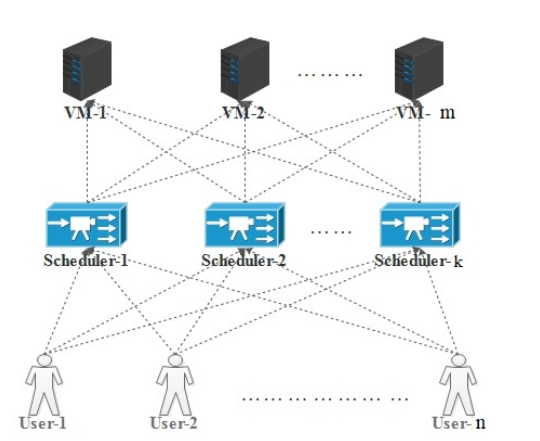
\includegraphics[width=0.3\textwidth, height=5cm]{Figures/Fig 1.png}
  \caption{System Model\cite{patra2019game}}
  \label{Fig 2}
\end{figure}

\subsection{Flowchart of the Algorithm}
The following algorithm was considered while modelling the game theoretic approach on this paper for task scheduling in cloud computing. A flowchart representation is shown on Figure \ref{Fig 1}
\begin{figure}[h]
  \centering
  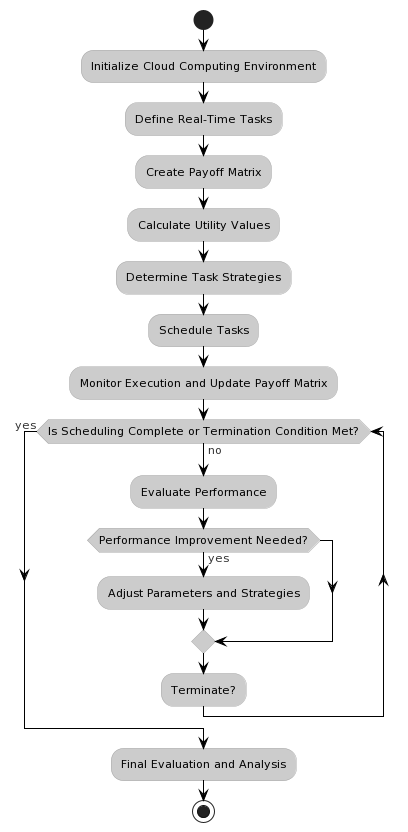
\includegraphics[width=0.35\textwidth, height=9cm]{Figures/Algorithom.png}
  \caption{Algorithm}
  \label{Fig 1}
\end{figure}


\bigskip
\section{\textbf{ GAME THEORETIC FRAMEWORK}}
The game formulation for real-time task scheduling is covered in this section. Game theory aims to forecast the best course of action for participants in a specific model by analyzing their relationships. A game is an interaction between several players in which the outcomes of individual players are influenced by the choices made by other players. In a game, there are a certain number of players, a predetermined set of strategies for each player, and a payoff that indicates whether each player wins or loses. We will have a look at different components of a game model :

• \textbf{Player}: An active participant in the game who makes strategic decisions.

• \textbf{Strategy}: It specifies how players will act in a specific situation.

• \textbf{Payoff}: It calculates a player's gains or losses based on a specific game result.

As discussed earlier, game theory has two main branches namely; (i) Co-Operative Game and (ii) Non Cooperative Game.
Both Cooperative and Non cooperative game will be considered here for real time task scheduling. Some of the attributes of the proposed game model are following :

\textbf{Player}: Each task is taken as a player i.e. $t_{i}$ = $p_{i}$. The set of player is represented by
$P = \{p_i \,|\, 1 \leq i \leq n\}$

\textbf{Strategies}: Every virtual machine functions as a strategy. To maximize their payoff, each player will look for the best strategy $v_{j}$.

\textbf{Payoff}: The variable payoff that $t_{i}$ will acquire while choosing a strategy $v_{j}$ can either be completion time $c_{ij}$ or waiting time $w_{ij}$.

\textbf{Payoff Matrix}: The payoff matrix is a table with player-1's strategies represented in each row and player-2's strategies represented in each column. In the suggested method, player-1 represents time period $t_{1}$, and player-2 represents time period $t_{2}$. The strategy is shown by $v_{j}$, where j = \{1, 2, \ldots, m\}.
The payoff of $t_{1}$ is represented by the first number in each cell in the table, and $t_{2}$ is represented by the second number. Figure 2 illustrates a payoff matrix with $m = 3$ as an example. The payoff for $t_{1}$ is 2 and the payoff for $t_{2}$ is 1 if $t_{1}$ selects $v_{2}$ and $t_{2}$ selects $v_{3}$.
Following is a description of how to determine the best two-player strategies for the non-cooperative and cooperative games.

\begin{figure}[h]
  \centering
  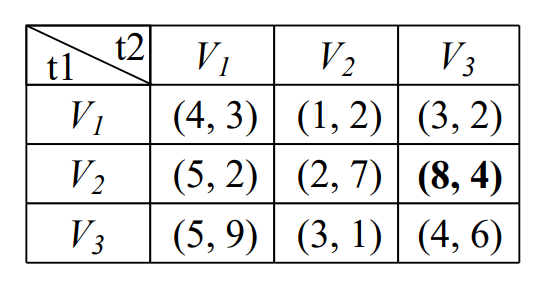
\includegraphics[width=0.4\textwidth, height=4cm]{Figures/PayoffMatrix.png}
  \caption{PayOff Matrix\cite{patra2019game}}
  \label{Fig 3}
\end{figure}

\begin{figure}[h]
  \centering
  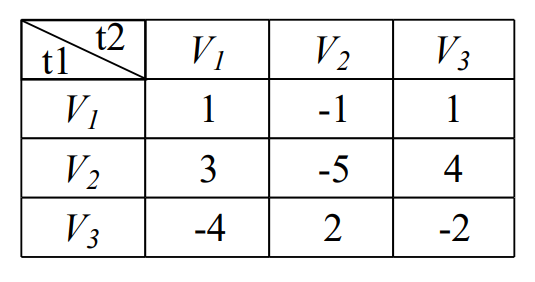
\includegraphics[width=0.4\textwidth, height=4cm]{Figures/Normalisedpayoff.png}
  \caption{Normalised PayOff Matrix\cite{patra2019game}}
  \label{Fig 4}
\end{figure}

\subsection{\textbf{Non- Cooperative Game}}
Let's take a look at the payoff matrix in Fig \ref{Fig 3}, which represents payoff as completion time. Every virtual machine's $t_{1}$ and $t_{2}$ completion times are calculated to create the payoff matrix. As shown in Fig \ref{Fig 4}, the payoff matrix is transformed into a normalized payoff matrix M by deducting the payoff of $t_{2}$ from the payoff of $t_{1}$.
A gain to $t_{2}$ and a loss to $t_{1}$ result from a positive value in the normalized payoff matrix. A gain to $t_{1}$ and loss to $t_{2}$ if the value in the normalized payoff matrix is negative. As we already mentioned, the payoff in our game model could either be waiting time or completion time. As a result, the gain is maximized when the payoff value is minimum. Task $t_{1}$ will attempt to reduce the maximum loss in accordance with the minimax principle. Therefore, we will first determine the highest element in each row before choosing the lowest element as $vm_{1}$. The mathematical formula to determine the minimum value between the maximum value for each $t_{1}$ strategy is :

\begin{center}
$vm1 = \min_{\forall i} \left( \max_{\forall j} M[i][j] \right)$
\end{center}

In Figure \ref{Fig 5}, the Row-Max column shows the highest values for each row, and the lowest value is 1 for row $v_{1}$, making row $vm_{1}$ equal to 1.
Task $t_{2}$ will attempt to maximize the minimum gain in accordance with the maximin principle. Therefore, we will first determine the minimum element for each column before choosing the maximum element as $vm_{2}$. The formula to determine the maximum value among the minimum value for each $t_{2}$ strategy is
\begin{center}
    $vm2 = \max_{\forall j} \left( \min_{\forall i} M[i][j] \right)$
\end{center}
\begin{figure}[h]
  \centering
  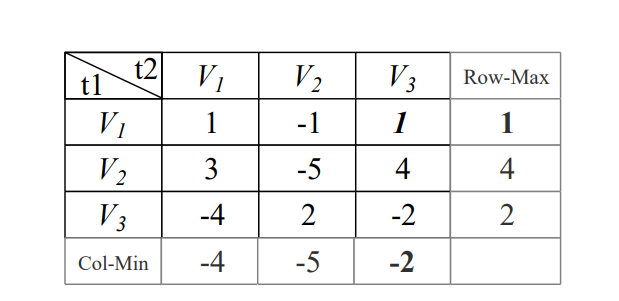
\includegraphics[width=0.4\textwidth, height=4cm]{Figures/Fig 4.png}
  \caption{VM Selection \cite{patra2019game}}
  \label{Fig 5}
\end{figure}
The Col-Min row in Fig. 4 shows the minimum values for each column, and the maximum value is -2 for $v_{3}$, meaning that $vm_{2}$ is -2.
The intersection point of $vm_{1}$ and $vm_{2}$ is then discovered; it is shown in Fig. 4 as 1 in italic bold. The chosen virtual machines will be $v_{1}$ for time $t_{1}$ and $v_{3}$ for time $t_{2}$. The same logic applies to rewards as it does to waiting times.

\subsection{\textbf{Cooperative Game}}
Let's assume that the payoff matrix in Figure \ref{Fig 6} represents payoff as completion time. By deducting the payoff of $t_{2}$ from the payoff of $t_{1}$, then taking the mode of that value, the cooperative game's payoff matrix is first transformed into a normalized payoff matrix.
The payoff matrix in Figure\ref{Fig 6} can be transformed into the normalized payoff matrix in Figure \ref{Fig 7}, which is displayed.
In the cooperative game, two players work together in the sense that they consider both their own and the other player's interests when making decisions. The normalized payoff matrix's large value denotes a significant difference in the gains of the two players, while the payoff matrix's small value denotes a relatively small difference in the gains of the two players. Therefore, excluding the diagonal elements, we are choosing the strategies (virtual machines) that correspond to the smallest value in the normalized payoff matrix. The smallest value is 1 in italic bold in Fig \ref{Fig 7}. So, $v_{3}$ for time $t_{1}$ and $v_{1}$ for time $t_{2}$ will be chosen as the corresponding virtual machines. The same rules apply to payoff as they do to waiting time $w_{ij}$.
\begin{figure}[h]
  \centering
  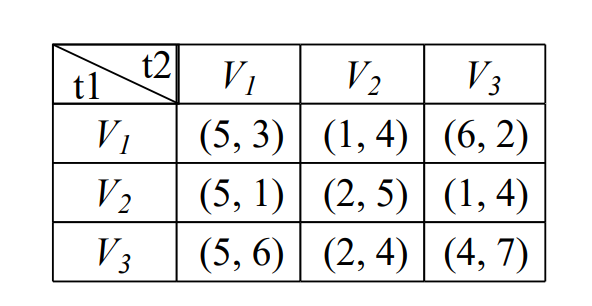
\includegraphics[width=0.4\textwidth, height=4cm]{Figures/Fig 5.png}
  \caption{Cooperative Payoff Matrix \cite{patra2019game}}
  \label{Fig 6}
\end{figure}


\begin{figure}[h]
  \centering
  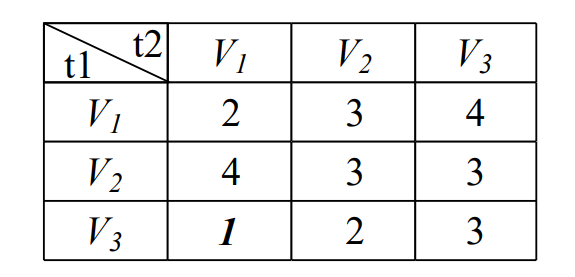
\includegraphics[width=0.4\textwidth, height=4cm]{Figures/Fig 6.png}
  \caption{Cooperative Normalised Payoff Matrix \cite{patra2019game}}
  \label{Fig 7}
\end{figure}


\bigskip
\section{\textbf{Results}}
Patra et. al 2009 \cite{patra2019game} conducted an experiment by taking different numbers of tasks ranging from 300 to 800, which are generated using a Poisson distribution, in order to show and prove that the proposed approach has an optimization result. Since the trend is the same for any number of tasks, the results of 500 tasks for both the non-cooperative and cooperative game models were discussed there. The following simulation settings and parameters were followed while conducting the experiment:

• Each virtual machine has a computing capacity that is set between [3000-6000] MIPS.

• Tasks are created by using the Poisson distribution to exponentially distribute inter arrival time.

• The task's due date is determined by the formula: 
$d_{li}$ = $a_{i}$ + $baseD$ ; where baseD belongs to the uniform distribution U (5, 10).

• The task's size has been set between 6000 and 10,000 MI.

The simulation results demonstrate that the cooperative game performs better because the tasks in non-cooperative games are selfish, meaning that players only consider their own benefits. One small task might have to wait for a bigger task for a very long time, increasing both the waiting time and the completion time. However, in the cooperative game, both tasks will work to cut down on waiting time and overall completion time.

\subsection{Completion Time as Payoff}
Here, Parta et. al 2009 presented \cite{patra2019game} experimental findings that allow players to view both cooperative and Non Cooperative game play performance as a reward. 10, 20, 30, 40, and 50 virtual machines are configured to run simultaneously. Figure \ref{Fig 8}  shows that a cooperative game model has a shorter total completion time than a non-cooperative game model.

\begin{figure}[h]
  \centering
  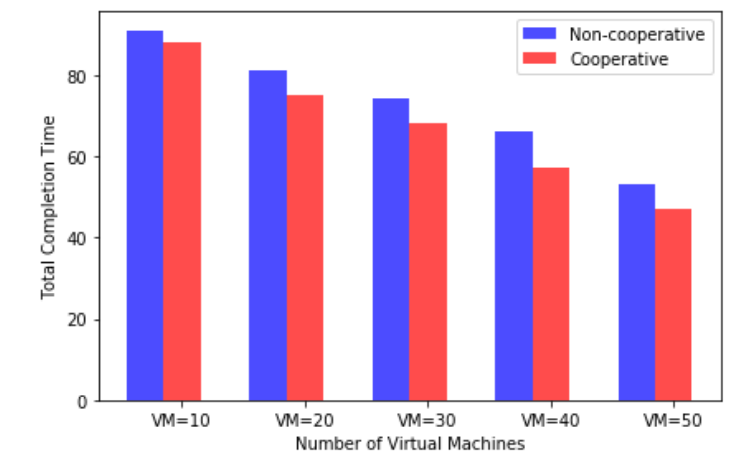
\includegraphics[width=0.4\textwidth, height=4cm]{Figures/Fig 7.png}
  \caption{Total Completion Time \cite{patra2019game}}
  \label{Fig 8}
\end{figure}

\subsection{Waiting Time as Payoff}
Here,Parta et. al 2009 presented \cite{patra2019game} experimental findings to understand how well cooperative and non-cooperative games performed when waiting time was the payoff. 10, 20, 30, 40, and 50 virtual machines are configured to run simultaneously. Figure \ref{Fig 9} show that a cooperative game model has a shorter total waiting time than a non-cooperative game model.

\begin{figure}[h]
  \centering
  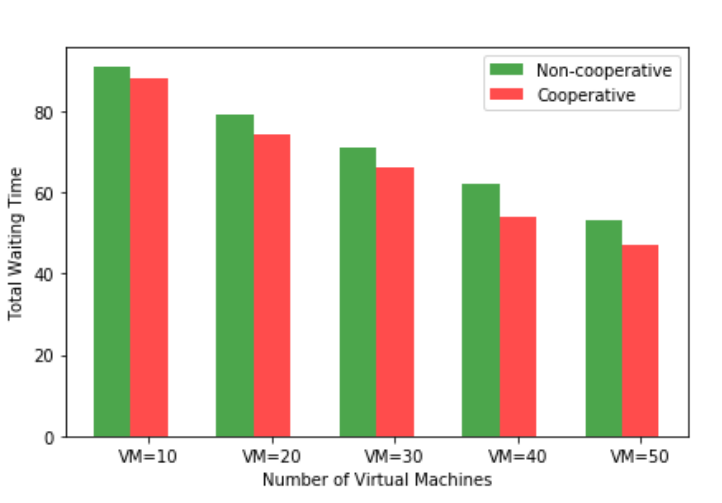
\includegraphics[width=0.4\textwidth, height=4cm]{Figures/Fig 8.png}
  \caption{Total waiting Time \cite{patra2019game}}
  \label{Fig 9}
\end{figure}

\bigskip
\section{\textbf{Conclusion and Future Work}}
Task scheduling is a critical aspect that requires careful consideration in the context of cloud computing. This paper proposes a game-theoretic method for real-time task scheduling in a cloud computing environment, utilizing both non-cooperative and cooperative game models. A comprehensive analysis of real-time task scheduling in cloud computing is presented, where user actions are treated as game players and virtual machines are considered as game strategies. A comparative analysis is conducted, examining the experimental results obtained from the cooperative and non-cooperative game models. The findings reveal that the cooperative game model for task scheduling outperforms the non-cooperative game model in terms of the chosen payoff metrics, namely completion time and waiting time. It is noteworthy that the total completion time and waiting time are consistently lower in the cooperative game model than in the non-cooperative game model, demonstrating the advantages of a cooperative approach.

Additionally, within the context of an IoT-based application model as described in\cite{patra2017architecture}, the application of a game-theoretic approach for load balancing is explored. This further highlights the applicability and effectiveness of game theory in addressing various challenges in cloud computing environments.

Moving forward, future research endeavors will encompass the integration of additional evaluation metrics, such as reliability and energy consumption, to enhance the proposed game-theoretic approach. By considering these factors, it is anticipated that the scheduling efficiency and overall performance of cloud computing systems can be further optimized.








\bibliography{Myref.bib}
\bibliographystyle{ieeetr}

\end{document}
